% =====================================================================
%  Fig. 1 -- End-to-end EfficientNet-GCN pipeline (two-column width)
% =====================================================================
\documentclass[tikz,border=3pt]{standalone}
\usepackage{helvet}
\renewcommand{\familydefault}{\sfdefault}
\usepackage{amsmath,amssymb}
\usetikzlibrary{arrows.meta,positioning,calc,fit,backgrounds,shapes.geometric,
                decorations.pathreplacing,patterns,shapes.misc}

\hyphenpenalty=10000 \exhyphenpenalty=10000 \pretolerance=10000 \tolerance=9999

\definecolor{cData}{HTML}{3D5A80}   \definecolor{cDataBg}{HTML}{E9EFF5}
\definecolor{cFroz}{HTML}{6C757D}   \definecolor{cFrozBg}{HTML}{E7E9EB}
\definecolor{cTrain}{HTML}{2A9D8F}  \definecolor{cTrainBg}{HTML}{DEF2EF}
\definecolor{cGraph}{HTML}{5B4B8A}  \definecolor{cGraphBg}{HTML}{ECE8F6}
\definecolor{cAux}{HTML}{BF7326}    \definecolor{cAuxBg}{HTML}{FBEEDA}
\definecolor{cFuse}{HTML}{9E2A2B}   \definecolor{cFuseBg}{HTML}{F8E5E5}
\definecolor{cXai}{HTML}{45774C}    \definecolor{cXaiBg}{HTML}{E5F0E6}
\definecolor{cInk}{HTML}{1F2933}

\newcommand{\prm}[2]{{\tiny\bfseries\textcolor{#1}{#2}}}

\begin{document}
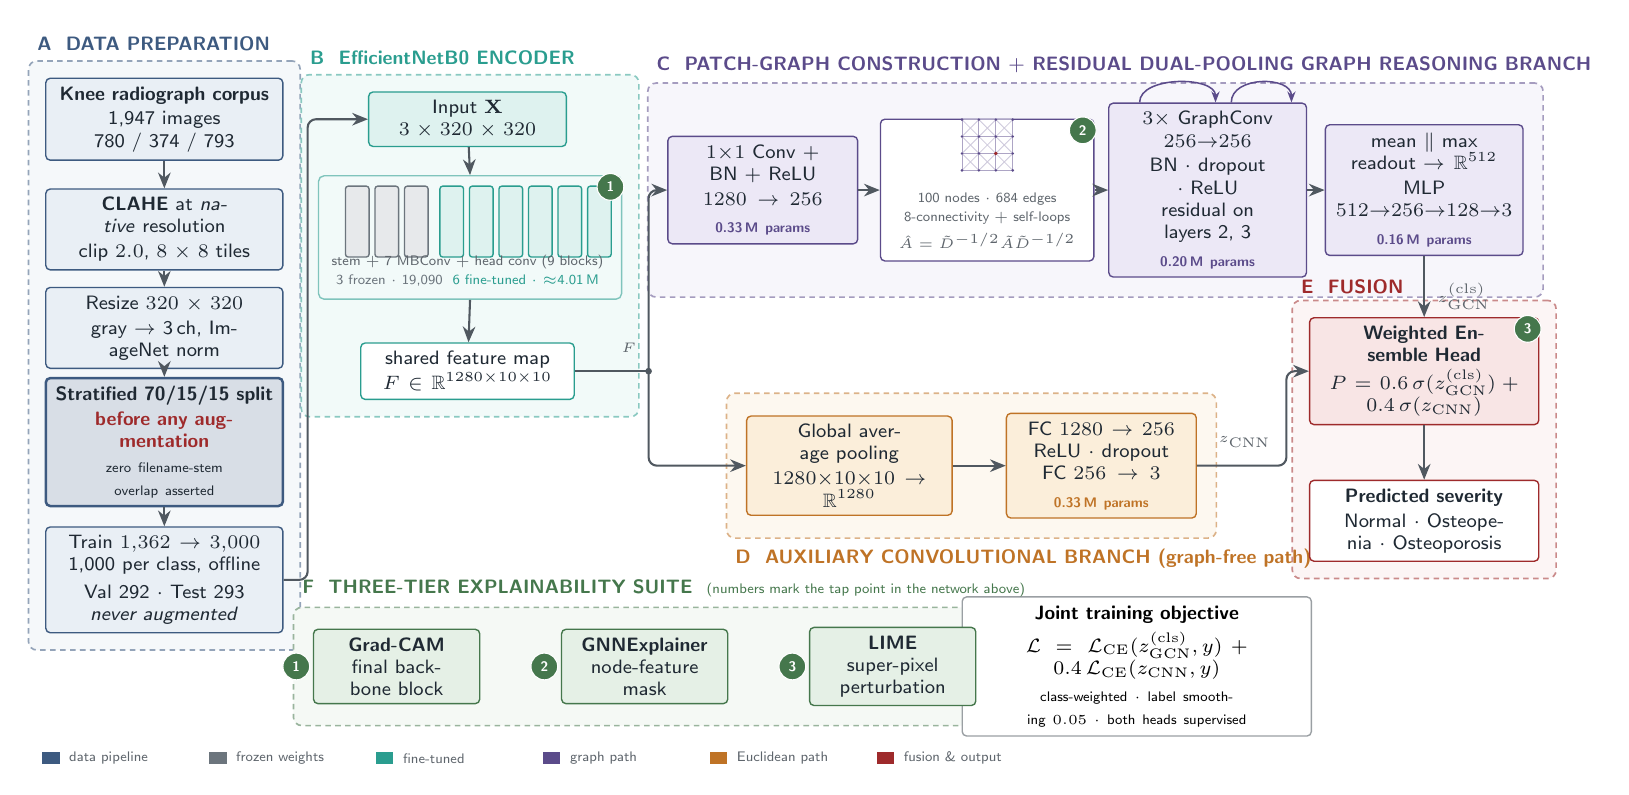
\begin{tikzpicture}[
  font=\scriptsize,
  blk/.style 2 args={draw=#1, fill=#2, rounded corners=1.6pt, line width=.5pt,
                     align=center, text=cInk, inner sep=3pt},
  lane/.style 2 args={draw=#1!55, fill=#2, rounded corners=3pt, line width=.6pt,
                      dash pattern=on 2pt off 1.6pt},
  lbl/.style={font=\scriptsize\bfseries, text=#1},
  flow/.style={-{Stealth[length=2mm,width=1.6mm]}, line width=.75pt, draw=cInk!78},
  route/.style={-{Stealth[length=2mm,width=1.6mm]}, line width=.75pt, draw=cInk!78,
                rounded corners=3pt},
  shp/.style={font=\tiny, text=cInk!72, inner sep=1pt},
  tapmk/.style={circle, fill=cXai, text=white, font=\tiny\bfseries,
                inner sep=0pt, minimum size=3.4mm, draw=white, line width=.4pt},
]

% ============ LANE A : DATA PREPARATION ============
\node[blk={cData}{cDataBg}, text width=28mm] (a1) at (0,8.45)
  {\textbf{Knee radiograph corpus}\\[1pt] 1{,}947 images\\ 780 / 374 / 793};
\node[blk={cData}{cDataBg}, text width=28mm] (a2) at (0,7.05)
  {\textbf{CLAHE} at \emph{native} resolution\\[1pt] clip $2.0$, $8\times8$ tiles};
\node[blk={cData}{cDataBg}, text width=28mm] (a3) at (0,5.80)
  {Resize $320\times320$\\[1pt] gray $\rightarrow$ 3\,ch, ImageNet norm};
\node[blk={cData}{cData!20}, text width=28mm, line width=.9pt] (a4) at (0,4.35)
  {\textbf{Stratified 70/15/15 split}\\[1pt]
   \textcolor{cFuse}{\textbf{before any augmentation}}\\[1pt]
   {\tiny zero filename-stem overlap asserted}};
\node[blk={cData}{cDataBg}, text width=28mm] (a5) at (0,2.60)
  {Train $1{,}362 \rightarrow 3{,}000$\\ 1{,}000 per class, offline\\[2pt]
   Val 292 $\cdot$ Test 293\\ \emph{never augmented}};
\foreach \s/\t in {a1/a2, a2/a3, a3/a4, a4/a5} \draw[flow] (\s) -- (\t);

\begin{scope}[on background layer]
  \node[lane={cData}{cDataBg!45}, fit=(a1)(a5), inner sep=6pt] (laneA) {};
\end{scope}
\node[lbl=cData, anchor=south west] at (laneA.north west) {A\ \ DATA PREPARATION};

% ============ LANE B : ENCODER ============
\node[blk={cTrain}{cTrainBg}, text width=23mm] (b0) at (3.85,8.45)
  {Input $\mathbf{X}$\\ $3\times320\times320$};

\foreach \i in {0,1,2}{
  \node[draw=cFroz, fill=cFrozBg, rounded corners=1pt, line width=.5pt,
        minimum width=3.0mm, minimum height=9mm] (fb\i) at (2.45+\i*0.375,7.15) {};}
\foreach \i in {0,1,2,3,4,5}{
  \node[draw=cTrain, fill=cTrainBg, rounded corners=1pt, line width=.5pt,
        minimum width=3.0mm, minimum height=9mm] (tb\i) at (3.65+\i*0.375,7.15) {};}
\node[shp, align=center] (bcap) at (3.85,6.53)
  {stem $+$ 7 MBConv $+$ head conv\ (9 blocks)\\[1pt]
   \textcolor{cFroz}{3 frozen $\cdot$ 19{,}090}\ \ \textcolor{cTrain}{6 fine-tuned $\cdot$ $\approx$4.01\,M}};
\node[draw=cTrain!60, rounded corners=2pt, line width=.5pt, fit=(fb0)(tb5)(bcap),
      inner sep=3.5pt] (bbox) {};
\node[tapmk] (t1) at ($(bbox.north east)+(-1.5mm,-1.5mm)$) {1};

\node[blk={cTrain}{white}, text width=25mm] (bF) at (3.85,5.25)
  {shared feature map\\[1pt] $F \in \mathbb{R}^{1280\times10\times10}$};

\draw[flow] (b0) -- (bbox.north);
\draw[flow] (bbox.south) -- (bF);

\begin{scope}[on background layer]
  \node[lane={cTrain}{cTrainBg!40}, fit=(b0)(bbox)(bF), inner sep=6pt] (laneB) {};
\end{scope}
\node[lbl=cTrain, anchor=south west] at (laneB.north west) {B\ \ EfficientNetB0 ENCODER};

\draw[route] (a5.east) -- (1.82,2.60) -- (1.82,8.45) -- (b0.west);

% ============ LANE C : GRAPH BRANCH ============
\node[blk={cGraph}{cGraphBg}, text width=22mm] (c1) at (7.60,7.55)
  {$1{\times}1$ Conv $+$ BN $+$ ReLU\\[1pt] $1280 \rightarrow 256$\\[2pt]
   \prm{cGraph}{0.33\,M params}};

\node[blk={cGraph}{white}, text width=25mm, minimum height=18mm] (c2) at (10.45,7.55) {};
\begin{scope}[shift={(10.13,7.80)}, scale=.215]
  \foreach \x in {0,1,2,3}\foreach \y in {0,1,2,3}{\coordinate (n\x\y) at (\x,\y);}
  \foreach \x in {0,1,2,3}\foreach \y in {0,1,2}{
    \draw[cGraph!50, line width=.34pt] (n\x\y) -- (n\x\the\numexpr\y+1\relax);}
  \foreach \x in {0,1,2}\foreach \y in {0,1,2,3}{
    \draw[cGraph!50, line width=.34pt] (n\x\y) -- (n\the\numexpr\x+1\relax\y);}
  \foreach \x in {0,1,2}\foreach \y in {0,1,2}{
    \draw[cGraph!30, line width=.3pt] (n\x\y) -- (n\the\numexpr\x+1\relax\the\numexpr\y+1\relax);
    \draw[cGraph!30, line width=.3pt] (n\x\the\numexpr\y+1\relax) -- (n\the\numexpr\x+1\relax\y);}
  \foreach \x in {0,1,2,3}\foreach \y in {0,1,2,3}{\fill[cGraph] (n\x\y) circle (2.4pt);}
  \fill[cFuse] (n21) circle (3.2pt);
\end{scope}
\node[shp, align=center] at (10.45,7.16)
  {100 nodes $\cdot$ 684 edges\\[1pt]
   8-connectivity $+$ self-loops\\[2pt]
   $\hat{A}=\tilde{D}^{-1/2}\tilde{A}\tilde{D}^{-1/2}$};
\node[tapmk] (t2) at ($(c2.north east)+(-1.5mm,-1.5mm)$) {2};

\node[blk={cGraph}{cGraphBg}, text width=23mm] (c3) at (13.25,7.55)
  {$3\times$ GraphConv $256{\to}256$\\[1pt] BN $\cdot$ dropout $\cdot$ ReLU\\
   residual on layers 2, 3\\[2pt]
   \prm{cGraph}{0.20\,M params}};
\draw[cGraph, line width=.55pt, -{Stealth[length=1.4mm]}]
  ($(c3.north west)+(4mm,0)$) .. controls +(0,3.4mm) and +(0,3.4mm) .. ($(c3.north)+(1mm,0)$);
\draw[cGraph, line width=.55pt, -{Stealth[length=1.4mm]}]
  ($(c3.north)+(3mm,0)$) .. controls +(0,3.4mm) and +(0,3.4mm) .. ($(c3.north east)+(-2mm,0)$);

\node[blk={cGraph}{cGraphBg}, text width=23mm] (c4) at (16.00,7.55)
  {mean $\Vert$ max readout $\rightarrow \mathbb{R}^{512}$\\[1pt]
   MLP $512{\to}256{\to}128{\to}3$\\[2pt]
   \prm{cGraph}{0.16\,M params}};

\foreach \s/\t in {c1/c2, c2/c3, c3/c4} \draw[flow] (\s) -- (\t);

\begin{scope}[on background layer]
  \node[lane={cGraph}{cGraphBg!40}, fit=(c1)(c2)(c3)(c4), inner sep=7pt] (laneC) {};
\end{scope}
\node[lbl=cGraph, anchor=south west] at (laneC.north west)
  {C\ \ PATCH-GRAPH CONSTRUCTION $+$ RESIDUAL DUAL-POOLING GRAPH REASONING BRANCH};

% ============ LANE D : AUXILIARY BRANCH ============
\node[blk={cAux}{cAuxBg}, text width=24mm] (d1) at (8.70,4.05)
  {Global average pooling\\[1pt] $1280{\times}10{\times}10 \rightarrow \mathbb{R}^{1280}$};
\node[blk={cAux}{cAuxBg}, text width=22mm] (d2) at (11.90,4.05)
  {FC $1280 \rightarrow 256$\\ ReLU $\cdot$ dropout\\ FC $256 \rightarrow 3$\\[2pt]
   \prm{cAux}{0.33\,M params}};
\draw[flow] (d1) -- (d2);

\begin{scope}[on background layer]
  \node[lane={cAux}{cAuxBg!40}, fit=(d1)(d2), inner sep=7pt] (laneD) {};
\end{scope}
\node[lbl=cAux, anchor=north west] at (laneD.south west)
  {D\ \ AUXILIARY CONVOLUTIONAL BRANCH (graph-free path)};

% feature-map fan-out
\draw[line width=.75pt, draw=cInk!78] (bF.east) -- (6.15,5.25);
\draw[route] (6.15,5.25) -- (6.15,7.55) -- (c1.west);
\draw[route] (6.15,5.25) -- (6.15,4.05) -- (d1.west);
\fill[cInk!78] (6.15,5.25) circle (1.2pt);
\node[shp] at (5.90,5.55) {$F$};

% ============ LANE E : FUSION ============
\node[blk={cFuse}{cFuseBg}, text width=27mm] (e1) at (16.00,5.25)
  {\textbf{Weighted Ensemble Head}\\[2pt]
   $P=0.6\,\sigma(z^{(\mathrm{cls})}_{\mathrm{GCN}})+0.4\,\sigma(z_{\mathrm{CNN}})$};
\node[tapmk] (t3) at ($(e1.north east)+(-1.5mm,-1.5mm)$) {3};
\node[blk={cFuse}{white}, text width=27mm] (e2) at (16.00,3.35)
  {\textbf{Predicted severity}\\[1pt] Normal $\cdot$ Osteopenia $\cdot$ Osteoporosis};

\draw[flow] (c4.south) -- (e1.north);
\draw[route] (d2.east) -- (14.25,4.05) -- (14.25,5.25) -- (e1.west);
\draw[flow] (e1) -- (e2);
\node[shp, anchor=west] at (16.13,6.20) {$z^{(\mathrm{cls})}_{\mathrm{GCN}}$};
\node[shp, anchor=south] at (13.72,4.24) {$z_{\mathrm{CNN}}$};

\begin{scope}[on background layer]
  \node[lane={cFuse}{cFuseBg!40}, fit=(e1)(e2), inner sep=6pt] (laneE) {};
\end{scope}
\node[lbl=cFuse, anchor=south west] at ($(laneE.north west)+(0,-0.5mm)$) {E\ \ FUSION};

% ============ training objective ============
\node[draw=cInk!45, fill=white, rounded corners=1.6pt, line width=.5pt,
      align=center, text width=42mm] (loss) at (12.35,1.50)
  {\textbf{Joint training objective}\\[2pt]
   $\mathcal{L}=\mathcal{L}_{\mathrm{CE}}(z^{(\mathrm{cls})}_{\mathrm{GCN}},y)
    +0.4\,\mathcal{L}_{\mathrm{CE}}(z_{\mathrm{CNN}},y)$\\[2pt]
   {\tiny class-weighted $\cdot$ label smoothing $0.05$ $\cdot$ both heads supervised}};

% ============ LANE F : EXPLAINABILITY ============
\node[blk={cXai}{cXaiBg}, text width=19mm] (x1) at (2.95,1.50)
  {\textbf{Grad-CAM}\\ final backbone block};
\node[tapmk] at ($(x1.west)+(-2.1mm,0)$) {1};
\node[blk={cXai}{cXaiBg}, text width=19mm] (x2) at (6.10,1.50)
  {\textbf{GNNExplainer}\\ node-feature mask};
\node[tapmk] at ($(x2.west)+(-2.1mm,0)$) {2};
\node[blk={cXai}{cXaiBg}, text width=19mm] (x3) at (9.25,1.50)
  {\textbf{LIME}\\ super-pixel perturbation};
\node[tapmk] at ($(x3.west)+(-2.1mm,0)$) {3};

\begin{scope}[on background layer]
  \node[lane={cXai}{cXaiBg!40}, fit=(x1)(x2)(x3), inner sep=7pt] (laneF) {};
\end{scope}
\node[lbl=cXai, anchor=south west] at (laneF.north west)
  {F\ \ THREE-TIER EXPLAINABILITY SUITE
   \ \textnormal{\tiny(numbers mark the tap point in the network above)}};

% ============ legend ============
\begin{scope}[shift={(-1.55,0.26)}]
  \foreach \i/\c/\t in {0/cData/{data pipeline}, 1/cFroz/{frozen weights},
                        2/cTrain/{fine-tuned}, 3/cGraph/{graph path},
                        4/cAux/{Euclidean path}, 5/cFuse/{fusion \& output}}{
    \fill[\c] (\i*2.12,0) rectangle ++(0.22,0.15);
    \node[shp, anchor=west] at (\i*2.12+0.30,0.075) {\t};}
\end{scope}

\end{tikzpicture}
\end{document}
